\section{Method}
\label{sec:metodo}

In order to build the knowledge graph of the semantic relationships between 
the objects found in a certain close environment of human occupation, such as 
a room, a deductive database \cite{stichbury}, we used Grakn.

Grakn is an Open Source engine for creating knowledge graphs that allow the 
user to organize and model complex data networks using the Entity-Relationship 
scheme in its maximum expressiveness. The architecture of Grakn is basically 
made up of two parts, as shown in Figure \ref{fig:arch}: \textit{Grakn} 
(the storage) and \textit{Graql} (the language).

\begin{figure}[H]
    \centering
    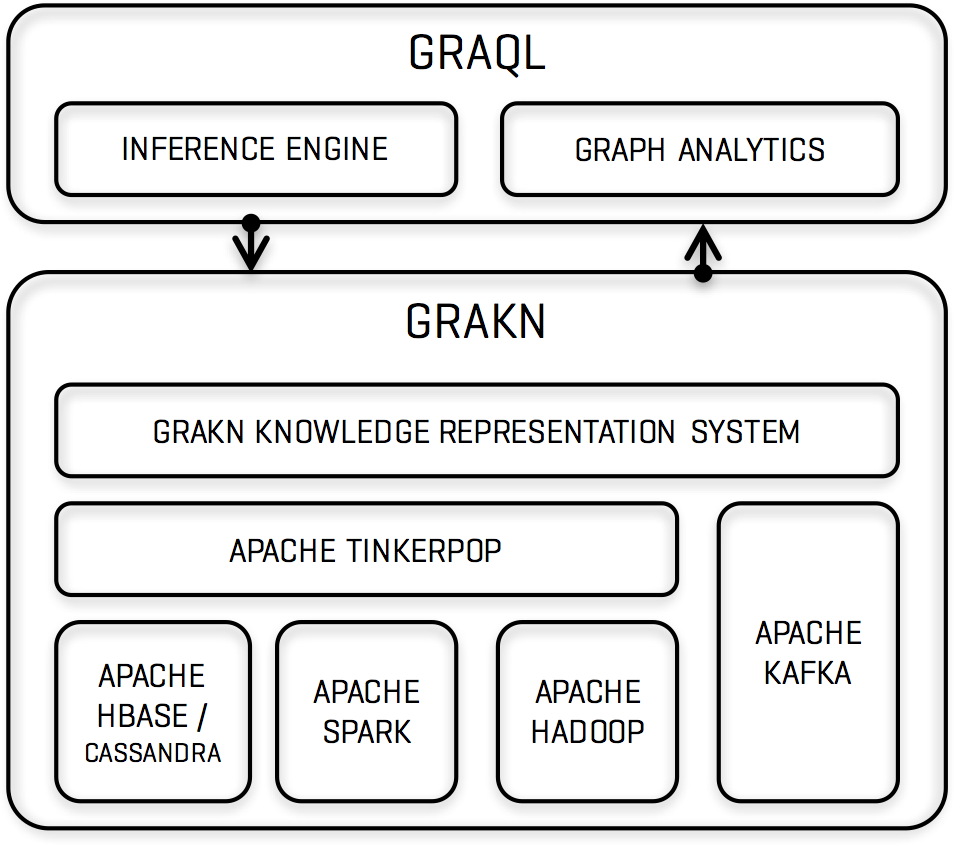
\includegraphics[width=6.8cm]{figures/architecture}
    \caption{Internal architecture of Grakn.
    Source \cite{stichbury}.}
    \label{fig:arch}
\end{figure}

In general, \textit{Grakn} can be seen as a distributed, hyper-relational 
database that uses intuitive\footnote{Refers to the definition of types, 
properties and relationships between existing entities in a given context.} 
ontology\footnote{It should not be seen from the side of philosophy, but as a 
branch of computer science.}  to model complex data, which serves as a 
knowledge base for cognitive systems \cite{dbengines}. 
%% Fig description
In figure \ref{fig:arch}, at the bottom we can see the Grakn system layer, 
which is made of Apache technologies: %
i) \textit{HBase}\footnote{Cassandra database servers the same purposes. It is 
a non-relational database that is distinguished by its speed, scale, 
and simplicity in design.} is a distributed, scalable, big data store databse, 
ii) \textit{Spark} for distributed processing system used for 
big data workloads.
iii) \textit{Hadoop} allows us to hanlde distributed processing of large data 
sets across clusters of computers using simple programming models.
This 3 technologies are the tools for \textit{Tinkerpop} to create the graph 
structure. At the right side of figure \ref{fig:arch} we have \textit{Kafka},
and its main function is to help the Grakn software to make graph data analytics
On the other hand, at the top of figure \ref{fig:arch} we have
\textit{Graql},it can be seen as a wrapper or friendly interface of the Grakn
system layer. Formaly, it is a knowledge-oriented declarative graph query 
language that retrieves knowledge in a explicit or implicit way.

Grakn was designed to be integrated with other technologies that allow it to 
function in a distributed manner. In addition, it is a great complement to 
Natural Language Processing (NLP) and Machine Learning (ML) systems 
\cite{grakn-youtube}.

Since Grakn creation in 2016 to present-day, it is use by several international 
companies, such as: Google and Cisco; and by institutions like MIT, OpenCTI, 
and Cares Genetics. Table \ref{fig:grakn-car} summarizes the most important 
features reported by the db-engines \cite{dbengines} site. A more detailed 
explanation can be found on the official Grakn site (\url{https://grakn.ai/}).

\begin{table}[H]
\caption{Grakn main features}
\begin{adjustbox}{width=\columnwidth,center}
\begin{tabular}{|l|l|}
\hline
\textbf{Feature}             & \textbf{Description}                   \\ \hline
Database model                      & Graph DBMS  and relational DBMS \\ \hline
Initial release                     & 2016                            \\ \hline
Current version                     &  1.7.2, June 2020            \\ \hline
Origin country                      & United Kingdom               \\ \hline
License                             & Open Source                  \\ \hline
Implementing language               & Java                         \\ \hline
Supporting operative systems        & Linux, OS X and Windows      \\ \hline
Triggers                            & no                            \\ \hline
Supporting languages                & 
\begin{tabular}[c]{@{}l@{}}All languages base on JVM:
\\ Groovy,\\ Java,\\ JavaScript (Node.js),\\ Python,\\Scala\end{tabular}\\\hline
APIS and other access methods       & 
\begin{tabular}[c]{@{}l@{}}Console (shell),\\ 
gRPC protocol,\\ Workbase (visualisation software)\end{tabular}      \\ \hline
Technical docs                      & https://dev.grakn.ai/­doc         \\ \hline
Usually compare with                & Neo4j, GraphDB y JanusGraph     \\ \hline
\end{tabular}
\end{adjustbox}
\label{fig:grakn-car}
\end{table}

\subsection{Grakn installation} % (fold)

To install Grakn, Java 8 SDK is previously required, if not you can download 
Oracle or OpenJDK implementation. To install Grakn in Linux we can use three 
package managers: \texttt{dnf}, \texttt{yum} (for systems that uses RPM
\footnote{RPM is a recursive acronym which means RPM Package Manager}) 
and \texttt{apt}.

Besides, Grakn is also available for X OS operative system,  through 
\texttt{brew} package manager. The testing implementations presented in the 
paper were made using CentOS 8.2 and Manjaro Linux 20.0.

Another important point is that Grakn works similarly to database management 
systems, which means we must start services, create users, workspaces, 
among others. In Grakn the abstract models that encapsulate 
the entities of a particular problem are known as \textit{Keyspace}, where the 
\textit{schemes} that will represent the data of the case study are defined.

An \textit{scheme} is an inherent part of the knowledge graph that describes 
what data is like and how it can be structured. It can be represented by an 
Entity-Relationship diagram. On the other side, Grakn has various types that 
made up the core system and provide the vocabulary necessary to describe any 
case study. The most important Grakn data types are:

\begin{itemize}
    \item \textit{Entities}. They provide the means to classify the objects of 
    a given domain.
    \item \textit{Relationships}. They connect the elements, known in Grakn as 
        \textit{things} from a particular domain. They can be objects, 
        relationships y attributes.
    \item \textit{Attributes}. They describe the entities.
\end{itemize}

Likewise, it is important to mention that the query language \textit{Graql} 
has the following characteristics:

\begin{itemize}
    \item \textit{Declarative}. In order to make a query with Graql, it may 
        describe what you want to recover, instead of saying how it should be 
        obtained.
    \item \textit{Intuitive}. Graql was designed to provide a high-level 
        query language interface with clear, readable syntax.
\end{itemize}

The operations that can be performed through Graql are data manipulation (DML) 
and data definition (DDL).

\subsection{Semantic relationship schema}
The semantic characterization created in this work is based on the following 
structure: \texttt{object1--predicate--object2} proposed by \cite{Cewu}, who 
points out that visual relationships capture a wide variety of interactions 
between pairs of objects in images. Therefore, it is recommended to extract the 
possible relationships that may exist, in order to reduce them and work more 
efficiently. Besides, the relations between each pair of objects must 
have a individual predicate, and based on this a classification is made 
to generate a relation. The most common types of predicates are classified 
by an action, space, a preposition, a comparison, or a verb as seen in Figure 
\ref{fig:predaCar}.

\begin{figure}[H]
    \centering
    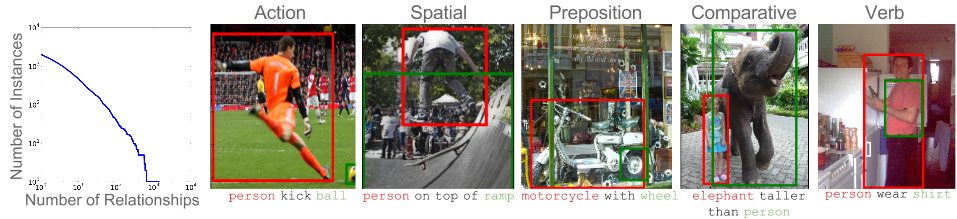
\includegraphics[width=8.8cm]{figures/predica.png}
    \caption{Predicates categorized. Source \cite{Cewu}.}
    \label{fig:predaCar}
\end{figure}

Based on the above, We use the spatial predicates for object characterization, 
since the objects belongs to certain human occupation space, 
such as a room, are static. Whereas, in this case, 
predicates based on verbs (actions) were not useful. In the Figures from 
\ref{fig:abelow} to \ref{fig:topUnder} the relationships used to make the 
knowledge graph are shown.

\begin{figure}[H]
    \centering
    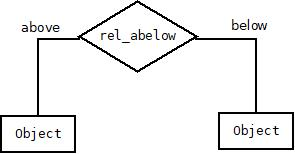
\includegraphics[width=5cm]{figures/abelow.jpg}
    \caption{Relation above-below.}
    \label{fig:abelow}
\end{figure}

\begin{figure}[H]
    \centering
    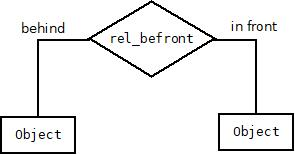
\includegraphics[width=5cm]{figures/befront.jpg}
    \caption{Relation behind-inFront.}
    \label{fig:befront}
\end{figure}

\begin{figure}[H]
    \centering
    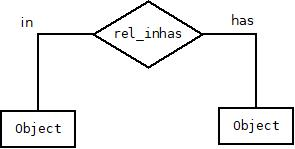
\includegraphics[width=5cm]{figures/inhas.jpg}
    \caption{Relation in-has.}
    \label{fig:inhas}
\end{figure}

\begin{figure}[H]
    \centering
    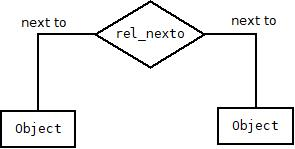
\includegraphics[width=5cm]{figures/nextto.jpg}
    \caption{Relation nextTo.}
    \label{fig:nexto}
\end{figure}

\begin{figure}[H]
    \centering
    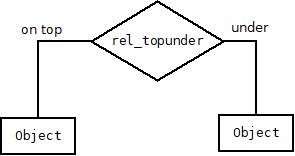
\includegraphics[width=5cm]{figures/topunder.jpg}
    \caption{Relation onTop-under.}
    \label{fig:topUnder}
\end{figure}

The elements recognize as objects have two attributes which are the identifier 
(ID) and the name as shown in Figure \ref{fig:object}. However, as more 
predicates are incorporated, it is possible to add more attributes to the 
object in order to better describe the relationship.

\begin{figure}[H]
    \centering
    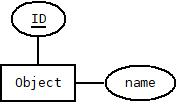
\includegraphics[width=4cm]{figures/object.jpg}
    \caption{Object attributes.}
    % \caption{Atributos de un objeto.}
    \label{fig:object}
\end{figure}

Before implementing the knowledge graph with Grakn, we drafted it, 
to visually identify the relationships that must be created through 
the tool. This conceptual design is seen in Figure \ref{fig:grafo}.

\begin{figure}[H]
    \centering
    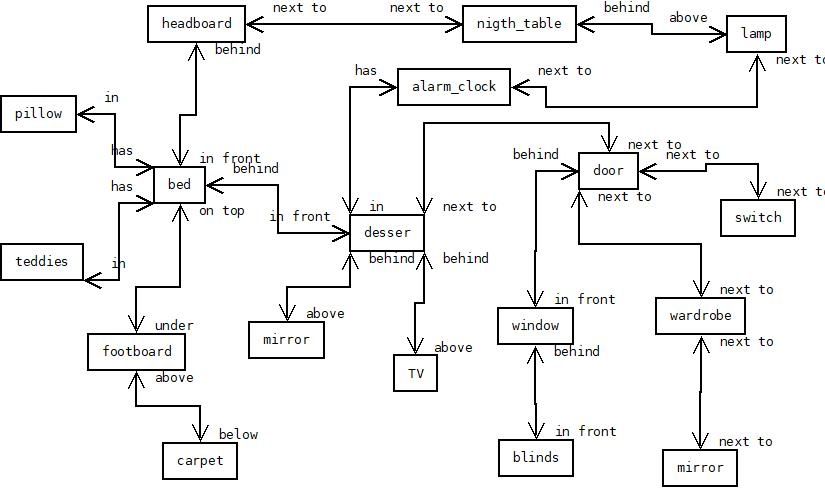
\includegraphics[width=8.8cm]{figures/grafo.jpg}
    \caption{Conceptual design of the knowledge graph.}
    \label{fig:grafo}
\end{figure}

\subsection{Development}

The implementation of the knowledge graph in Grakn was based on the previously 
defined relationships scheme, shown in the previous section. Thus, with the 
help of the Graql language, relations of type \texttt{above-below} were defined 
first and then the object, as can be seen in Listing \ref{lst:script1} and 
\ref{lst:script2}, respectively.

\lstinputlisting[language=Python, firstline=1, lastline=8,
    caption=Relationship definition using Graql.,
    label={lst:script1}
]{code/schema.gql}

\lstinputlisting[language=Python, firstline=22, lastline=35,
caption=Object definition using Graql., label={lst:script2}]{code/schema.gql}

Later, another script was created to insert the objects, as well as to insert 
the relationships that exist between them. It should be noted that the 
identifier is assigned automatically, so it is not necessary to declare 
it when inserting it. The insertion of the objects is done with the reserved 
word \textit{insert} and the relations with the combination of words 
\textit{insert} and \textit{match}, as seen in Listing \ref{lst:script3} and 
\ref{lst:script4}. A total of seventeen objects were inserted.

\lstinputlisting[language=Python, firstline=1, lastline=2,
caption=Object insertion., label={lst:script3}]{code/data.gql}

\lstinputlisting[language=Python, firstline=62, lastline=65,
caption=Object relationship., label={lst:script4}]{code/data.gql}

On the other side, to execute the code it was necessary to create a dedicated 
\textit{keyspace}, which was named \texttt{vision\_relationships}, where the 
schemes and relationships were made. Finally, to check that the objects have 
been inserted correctly, a query was made via console, as shown in Figure 
\ref{fig:correct}. Thus, the created objects were also counted.

\begin{figure}[H]
     \centering
     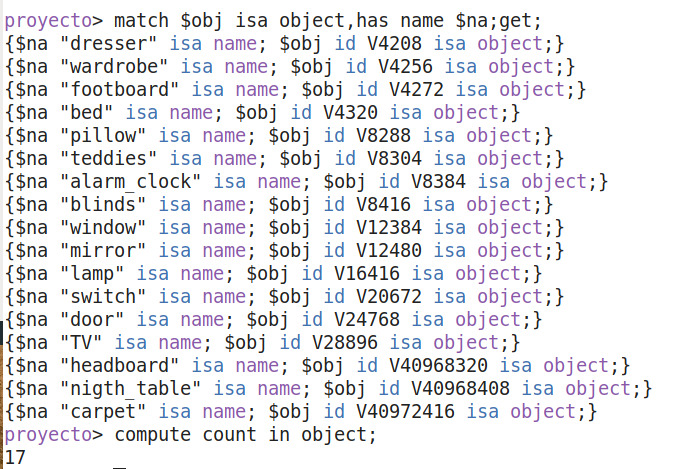
\includegraphics[width=8.8cm]{figures/numObje.jpeg}
     \caption{Query to check that there are no errors.}
     \label{fig:correct}
\end{figure}